\section{Introduction}

RAVEN (Risk Analysis Virtual ENvironment) \cite{raven, RAVENuserManual} is a framework for risk- and
uncertainty-based stochastic analysis. % TODO say more

Occasionally, the applications of RAVEN become sufficiently varied and complex to warrant a special application to a particular suite of problems. These special applications may introduce new physics, new templates, new RAVEN entities, or any combination of the above. In this instance, it's worth considering whether developing a Plugin could be beneficial to you and the community.

\subsection{What are Plugins?}

Plugins are defined the RAVEN Software Quality Assurance documentation \cite{RAVENuserManual}. They are intended to allow development that does not fit in the scope of RAVENs mission to be completed in a way that is still captured under the umbrella of RAVEN-based tools.

\subsection{What isn't a Plugin?}

While Plugins have wide applicability to extending the functionaliy of RAVEN, there are some alternatives that may be more suitable for some developments.

A Plugin is not simple a RAVEN Template. RAVEN Templates are used to simplify complex RAVEN workflows for more restrictive but increasingly efficient workflow permutations. If the end result of development is only a new RAVEN Template, we recommend you contribute this as a new templated workflow rather than a separate Plugin.

A Plugin is not a set of models that do similar activities to what RAVEN already does. For example, if new development includes RAVEN postprocessors and RAVEN metrics for uncertainty analysis and clustering using a particular theory, this is well within RAVENs scope and should be directly contributed to the code so these additions can benefit the community directly without the Plugin interaction.

\subsection{How do I decide?}

Ultimately, the decision to develop a plugin is best discussed with the RAVEN core team. However, the following guidelines may help inform a good decision.

\begin{figure}[h!]
  \centering
  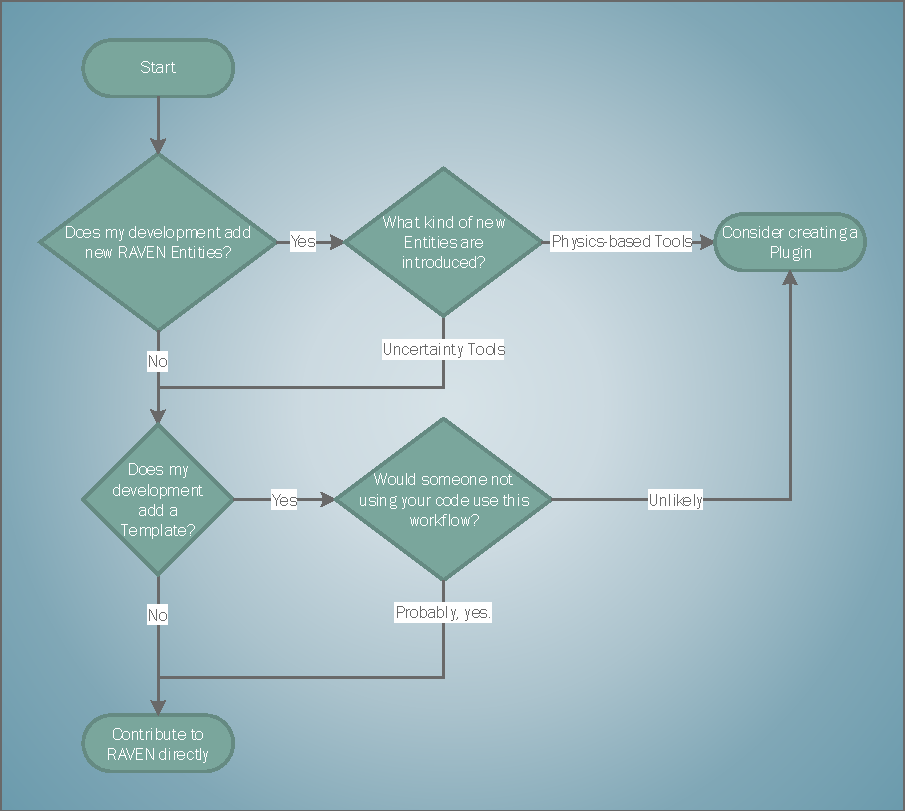
\includegraphics[scale=0.7]{pics/toPluginOrNot.pdf}
  \caption{Choosing to Plugin Workflow}
  \label{fig:choose plugin}
 \end{figure}

 \subsection{Supported Plugins}

 Officially supported RAVEN Plugins are a subset of all Plugins filtered by a particular set of characteristics. It is intended that all official Plugins are compatible with the latest developments in RAVEN as well as with each other. Additionally, official plugins contain continuous integration (CI) testing and provide the necessary software quality assurance (SQA) documentation to be included in RAVEN's SQA plan.

 To be an officially supported RAVEN Plugin, the following prerequesites must be met:
 \begin{itemize}
  \item The appropriate SQA documentation for NQA-1 level 2 coverage under the RAVEN SQA must be in place for the Plugin.
  \item The Plugin must contain CI testing with coverage consistent with RAVEN SQA. This CI testing must be compatible with RAVEN's CI testing system.
  \item The Plugin must contain documentation explaining the use and options included in the Plugin's contents.
  \item If at any time a change in RAVEN causes a failure in the CI tests in the plugin, the plugin must be updated to be compatible with the new RAVEN.
 \end{itemize}

 If a Plugin fails any of these criteria, a grace period (usually a month) is provided along with
 notification to the Plugin developers. If the grace period expires and the Plugin does not meet the
 requirements, it may be removed from the official supported Plugins list, pending an update to the
 Plugin.

